\documentclass[10pt]{exam}

\usepackage{amssymb, amsmath, amsthm, mathrsfs, multicol, graphicx}
\usepackage{tikz}

 \def\d{\displaystyle}
\def\?{\reflectbox{?}}
\def\b#1{\mathbf{#1}}
\def\f#1{\mathfrak #1}
\def\c#1{\mathcal #1}
\def\s#1{\mathscr #1}
\def\r#1{\mathrm{#1}}
\def\N{\mathbb N}
\def\Z{\mathbb Z}
\def\Q{\mathbb Q}
\def\R{\mathbb R}
\def\C{\mathbb C}
\def\F{\mathbb F}
\def\A{\mathbb A}
\def\X{\mathbb X}
\def\E{\mathbb E}
\def\O{\mathbb O}
\def\U{\mathcal U}
\def\pow{\mathcal P}
\def\inv{^{-1}}
\def\nrml{\triangleleft}
\def\st{:}
\def\~{\widetilde}
\def\rem{\mathcal R}
\def\sigalg{$\sigma$-algebra }
\def\Gal{\mbox{Gal}}
\def\iff{\leftrightarrow}
\def\Iff{\Leftrightarrow}
\def\land{\wedge}
\def\And{\bigwedge}
\def\AAnd{\d\bigwedge\mkern-18mu\bigwedge}
\def\Vee{\bigvee}
\def\VVee{\d\Vee\mkern-18mu\Vee}
\def\imp{\rightarrow}
\def\Imp{\Rightarrow}
\def\Fi{\Leftarrow}

%\def\={\equiv}
\def\var{\mbox{var}}
\def\mod{\mbox{Mod}}
\def\Th{\mbox{Th}}
\def\sat{\mbox{Sat}}
\def\con{\mbox{Con}}
\def\bmodels{=\joinrel\mathrel|}
\def\iffmodels{\bmodels\models}
\def\dbland{\bigwedge \!\!\bigwedge}
\def\dom{\mbox{dom}}
\def\rng{\mbox{range}}
\DeclareMathOperator{\wgt}{wgt}


\def\bar{\overline}


\newcommand{\vtx}[2]{node[fill,circle,inner sep=0pt, minimum size=4pt,label=#1:#2]{}}
\newcommand{\va}[1]{\vtx{above}{#1}}
\newcommand{\vb}[1]{\vtx{below}{#1}}
\newcommand{\vr}[1]{\vtx{right}{#1}}
\newcommand{\vl}[1]{\vtx{left}{#1}}
\renewcommand{\v}{\vtx{above}{}}

\def\circleA{(-.5,0) circle (1)}
\def\circleAlabel{(-1.5,.6) node[above]{$A$}}
\def\circleB{(.5,0) circle (1)}
\def\circleBlabel{(1.5,.6) node[above]{$B$}}
\def\circleC{(0,-1) circle (1)}
\def\circleClabel{(.5,-2) node[right]{$C$}}
\def\twosetbox{(-2,-1.4) rectangle (2,1.4)}
\def\threesetbox{(-2.5,-2.4) rectangle (2.5,1.4)}
\newcommand{\twoline}[2]{\begin{pmatrix}#1 \\ #2 \end{pmatrix}}


\def\circleA{(-.5,0) circle (1)}
\def\circleAlabel{(-1.5,.6) node[above]{$A$}}
\def\circleB{(.5,0) circle (1)}
\def\circleBlabel{(1.5,.6) node[above]{$B$}}
\def\circleC{(0,-1) circle (1)}
\def\circleClabel{(.5,-2) node[right]{$C$}}
\def\twosetbox{(-2,-1.5) rectangle (2,1.5)}
\def\threesetbox{(-2,-2.5) rectangle (2,1.5)}


%\pointname{pts}
\pointsinmargin
\marginpointname{pts}
\marginbonuspointname{pts-bns}
\addpoints
\pagestyle{head}
\printanswers

\firstpageheader{Math 228}{\textbf{Homework 4 Solutions}}{Due: September 19}


\begin{document}
\noindent \textbf{Instructions}: Same rules as usual.  Write up solutions on separate sheets of paper; you may work together to understand the problems, but write up your solutions individually.  You may NOT look for solutions online or in other books.

\begin{questions}

  \question[8] Find the largest number of points which a football team cannot get exactly using just 3-point field goals and 7-point touchdowns (ignore the possibilities of safeties, missed extra points, and two point conversions).  Prove your answer is correct by mathematical induction.  That is, find the largest impossible score (call it $m$) and prove that for any number $n > m$, it is possible to score $n$ points.

  \begin{solution}
    First note that it is impossible to make 11 points -- if only field goals are made, the points must be a multiple of 3, if 1 touchdown is made, the possible point totals are 7, 10, 13, \ldots and two touchdowns are already too much.

    We will prove that 11 is the largest number of points which cannot be made.  In other words, any number of points greater than or equal to 12 can be made.

    \begin{proof}
      Let $P(n)$ be the statement ``it is possible to make $n$ points using touchdowns and field goals.''  We will prove $P(n)$ is true for all $n \ge 12$.

      First the base case: You can make 12 points with 4 field goals, so $P(12)$ is true.

      Now the inductive case: Assume $P(k)$ is true for some fixed $k \ge 12$.  That is, it is possible to make $k$ points.  Since $k \ge 12$, we must have made the $k$ points using either at least 2 field goals or at least 2 touchdowns, or both (because if we used just one of each we would have only 10 points).  Now if the $k$ points were accomplished with 2 (or more) field goals, then replace 2 field goals with 1 touchdown.  This increases to point total by 1, giving $k + 1$ points.  On the other hand, if the $k$ points were accomplished with $2$ (or more) touchdowns, replace 2 touchdowns with 5 field goals, again increasing the point total by 1, giving $k+1$ points.  Using one of these two substitutions, we can make $k+1$ points, so $P(k+1)$ is true, establishing the inductive case.

      Therefore by the principle of mathematical induction, $P(n)$ is true for all $n \ge 12$.
    \end{proof}
  \end{solution}


  \question[8] Prove that the sum of the interior angles of a convex $n$-gon is $(n-2)\cdot 180^\circ$.  (A convex $n$-gon is a polygon with $n$ sides for which each interior angle is less than $180^\circ$.)  You may assume the fact that the interior angles of any triangle have sum $180^\circ$.

  Hint:
  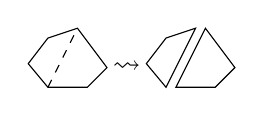
\begin{tikzpicture}[scale=0.5]
    \draw (0,0) -- (1,0) -- (1.5,.5) -- (.75,1.5) -- (0,1.25) -- (-.5,.6) -- cycle;
    \draw[dashed] (0,0) -- (.75,1.5);
    \node at (2,.5) {$\rightsquigarrow$};
        \draw (3.25,0) -- (4.25,0) -- (4.75,.5) -- (4,1.5)-- cycle;
        \draw (3,0) -- (3.75,1.5) -- (3,1.25) -- (2.5,.6) -- cycle;
  \end{tikzpicture}


  \begin{solution}
  Every $n$-gon (for $n \ge 4$) can be divided into two smaller polygons, a $j$-gon and a $k$-gon where $n = j-1 + k-1$ (since on each you are adding a new side). The sum of the interior angles of the $n$-gon will then be the sum of the angles in the two smaller polygons.  This suggests a proof by strong induction (you could do a proof by weak induction if you insist one of the two smaller polygons is a triangle, because then the other polygon will have $n-1$ sides).

  \begin{proof}
  Let $P(n)$ be the statement, ``the sum of the interior angles of a convex $n$-gon is $(n-2)\cdot 180^\circ$.''  We will prove $P(n)$ is true for all $n \ge 3$.

  Base case: When $n=3$, we have a triangle, and we know the sum of the interior angles of a triangle is $180^\circ = (3-2)\cdot 180^\circ$.  Thus $P(3)$ is true.

  Inductive case: Fix $k \ge 3$ and assume $P(j)$ is true for all $j \le k$.  That is, the sum of the angles of any convex $j$-gon is $(j-2)\cdot 180^\circ$.  Now consider an arbitrary convex $(k+1)$-gon.  Draw an edge between two non-adjacent vertices (for example, between the first and third vertices counting clockwise).  Since we have at least 4 vertices, this is possible, and divides the $k+1$-sided polygon into a convex $j$-gon and a convex $l$-gon, where $j-1+l-1 = k+1$.  The sum of the angles of the $(k+1)$-gon will be exactly the sum of the angles in the $j$-gon plus the sum of the angles in the $l$-gon.
  But the $j$-gon has sum of angles $(j-2)\cdot 180^\circ$ (by the inductive hypothesis) and the $l$-gon has sum of angles $(l-2)\cdot 180^\circ$, so together the sum of the interior angles of the $(k+1)$-gon is
  \[(k-2)\cdot 180^\circ + (l-2)180^\circ = (l+k-4)\cdot 180^\circ = (k+1-2)\cdot 180^\circ\]
  Since we can do this for \emph{any} convex $(k+1)$-gon, we see that $P(k+1)$ is true.

  Therefore, by the principle of mathematical induction, $P(n)$ is true for all $n\ge 3$.

  \end{proof}

  \end{solution}


  \question[8] Let $G$ be a connected graph with $v$ vertices and $e$ edges.  Use mathematical induction to prove that if $G$ contains exactly one cycle (among other edges and vertices), then $v = e$.  This is asking you to prove a special case of Euler's formula for planar graphs, so do not use that formula in your proof.  You should complete this proof in two parts:
  \begin{parts}
    \part First, prove, by induction, that the cycle $C_n$ has $v = e$.  You will need to think about how to get from $C_n$ to $C_{n+1}$.
    \begin{solution}
      Let $P(n)$ be the statement, ``The graph $C_n$ has the same number of edges as vertices.''  We will show $P(n)$ is true for all $n \ge 3$.  
      
      Base case: When $n = 3$, we are looking at the graph $C_3$ which consists of three vertices and three edges.  So $P(3)$ is true.
      
      Inductive case: Fix $k \ge 3$ and assume that $P(k)$ is true.  That is, $C_k$ has the same number of edges as vertices.  To form $C_{k+1}$, we can replace an edge by two edges with a vertex between them.  This increases the number of edges by 1, and also the number of vertices by 1, so we see that $C_{k+1}$ also has an equal number of edges and vertices.
      
      Therefore, by the principle of mathematical induction, $C_n$ has an equal number of edges and vertices, for all $n \ge 3$.
    \end{solution}
    \part Next, prove that for any $G$ with exactly one cycle, $v = e$.  Here you will want to start with an arbitrary graph $G$ with exactly one cycle, and consider two cases: either $G = C_n$, or not.
    \begin{solution}
      Let $P(n)$ be the statement, ``any graph with $n$ vertices that has exactly one cycle will have $n$ edges.''  We will prove $P(n)$ is true for all $n \ge 3$.
      
      Base case: When $n = 3$, the only graph with exactly one cycle is $C_3$, which has 3 edges.
      
      Inductive case: Fix $k \ge 3$ and assume $P(k)$ is true.  That is, every graph with $k$ vertices and exactly one cycle has $k$ edges.  Now consider an arbitrary graph $G$ with $k+1$ vertices and exactly one cycle.  If $G$ is just a cycle, then $G = C_{k+1}$, which has $k+1$ edges as seen in part (a).  If $G$ is not just a cycle, then there must be a vertex of degree 1 (you could prove this by removing the cycle from $G$ and looking at the longest path in what remains).  
      
      Let $v_0$ be a vertex of degree 1 in $G$ and let $G'$ be the graph you get by removing $v_0$ and its one incident edge.  $G'$ is a graph with exactly one cycle and $k$ vertices, so by the inductive hypothesis, $G'$ has $k$ edges.  But $G$ has one more edge than $G'$, so $G$ has $k+1$ edges.  This proves $P(k+1)$ is true.
      
      Therefore, by the principle of mathematical induction, $P(n)$ is true for all $n \ge 3$.
    \end{solution}
  \end{parts}


  \question[6] Use Euler's formula for planar graphs to answer the questions below.
  \begin{parts}
    %Next time, rephrase this.  A student thought it might mean that some edges could cross but the non-crossing edges create 4 faces.
    \part Is it possible to draw a connected graph with 7 vertices and 10 edges so that no edges cross creating 4 faces?  Explain.
    \begin{solution}
      No.  Such a graph would be planar (since you can draw it without edges crossing), and would have $v = 7$, $e = 10$ and $f = 4$.  But $7-10+4 = 1 \ne 2$, so this would violate Euler's formula.
    \end{solution}
    \part Is it possible for a graph with 10 vertices and 8 edges to be a connected planar graph?  Explain.
    \begin{solution}
      No.  Suppose it was.  Then the number of faces would satisfy $10 - 8 + f = 2$ which would mean there are 0 faces, an impossibility.
    \end{solution}
    \part Is there a connected planar graph with an odd number of faces where every vertex has degree 6?  Explain.
    \begin{solution}
      No.  Suppose there was such a graph.  Since every vertex has degree 6, there would be $e = \frac{6v}{2}$ edges (where $v$ is the number of vertices).  Then Euler's formula would say $v - \frac{6v}{2} + f = 2$.  This simplifies to $f = 2 + 2v$.  Since $v$ is an integer, we see that $f$ must therefore be even.
      
      Note that in fact, there is not even a connected planar graph in which every vertex has degree 6, not even with an even number of faces.  You could prove this by also considering the inequality $3f \le 2e$ which would become $3f \le 6v$ and thus $f \le 2v$, which cannot hold if $f = 2+2v$.
    \end{solution}
  \end{parts}




  \bonusquestion[5] Bonus: Given a square, you can cut the square into smaller squares by cutting along lines parallel to the sides of the original square (these lines do not need to travel the entire side length of the original square).  For example, by cutting along the lines below, you will divide a square into 6 smaller squares:
  \begin{center}
    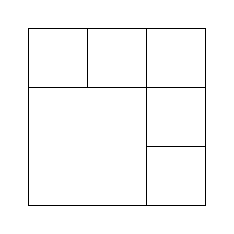
\begin{tikzpicture}[scale=.75]
      \draw (0,0) rectangle (3,3) (0,0) rectangle (2,2) (1,2) -- (1,3) (2,2) -- (2,3) (2,2) -- (3,2) (2,1)-- (3,1);
    \end{tikzpicture}
  \end{center}
  Prove, using strong induction, that it is possible to cut a square into $n$ smaller squares for any $n \ge 6$.  Hint: you will need three base cases.

  \begin{solution}
    It is possible to cut a square into 6, 7 and 8 squares.  Further, whenever you have cut a square into $n$ squares, it is possible to cut it into $n+3$ squares, by cutting one of the $n$ squares into 4 (you gain 4, but lose the one you cut up).  This allows you to state the inductive case as follows:
    
    Fix $k \ge 8$ and assume that $P(j)$ is true for all $6 \le j \le k$.  Now consider $P(k+1)$.  Since $k \ge 8$, we know that $k-2 \ge 6$, and thus we know that $P(k-2)$ is true.  That is, you can cut up a sqaure into $k-2$ squares.  Take one of these and cut it into 4 squares.  You will be left with $k+1$ squares total, so $P(k+1)$ is true.
  \end{solution}

\end{questions}




\end{document}
